\newpage
\section{Implementation}

For long code snippets, we recommend to put them into the appendix of the
report. However, do not forget to reference them in the text. Small code
snippets can also be put directly alongside the respective paragraphs.

\subsection{Resources}

This section is supposed to enumerate (at least) \emph{four} helpful resources
that you conducted during implementation (e.g., the official documentation of
the chosen system). Briefly discuss in which respect the respective resources
were useful (1 paragraph each).

Although not mandatory, we would like to encourage you to list \emph{all}
resources that were useful to you (even without description).

\begin{packed_enum}
   \item \ldots
   \item \ldots
   \item \ldots
   \item \ldots
   \item Additional resource \ldots
\end{packed_enum}

\subsection{Setup}

Describe the machine setup thoroughly. This section serves as documentation of
your setup such that someone else could read through it and deploy your
application on a different machine after configuring this machine accordingly.
This includes (but is not limited to) the operating system of your (virtual)
machine, third-party tools/libraries, or modifications to configuration files.
Also explain why the respective tools/modifications were required/necessary in
order to get your application running (or maybe you just used/modified them for
convenience, which would also be okay).


We used an instance of Amazon's EC2 Server\footnote{https://aws.amazon.com/de/ec2/}. The server's free trial period lasts for one year, so no fees were charged. We deployed an Ubuntu 16.04 LTS\footnote{http://releases.ubuntu.com/16.04/} instance to the server. When the creation is finished, you receive a SSH-Key for the default user (ubuntu). You can use this key to log into the server.

\subsubsection{General Setup}
\label{sec:setup}
At first we will update the package-list, the packages itself and the distribution. After that we will clean up the installation. For this procedure the following commands are used.
\begin{lstlisting}
sudo apt-get update
sudo apt-get upgrade
sudo apt-get dist-upgrade
sudo apt-get autoremove
\end{lstlisting}

With the following commands for each team member (kard, sprs, schf) an user is created, sudo access granted and a SSH key pair generated. The following process can be repeated for any user. 
\\\\
Creates an user, \textit{-m} creates a home directory for that user too.
\begin{lstlisting}
sudo useradd -m kard
\end{lstlisting}

Grants root access to the given user.
\begin{lstlisting}
sudo usermod -a -G sudo kard
\end{lstlisting}

Sets a password for the given user, this could be any string generated with random.org, \textit{-e} states that the user has to change the password during his or her next login.
\begin{lstlisting}
sudo passwd kard -e
\end{lstlisting}

The following statement generates a key pair which will later be used to login and needs to be executed on the client as the generated private key should not pass the network (also make sure that ssh-keygen is installed).
\begin{lstlisting}
ssh-keygen nsdb-aws-kard
\end{lstlisting}

Next we will create an \textit{.ssh} directory in the user's home directory and create a file with the authorized keys in it, which will now be empty.
\begin{lstlisting}
mkdir .ssh
touch .ssh/authorized_keys
\end{lstlisting}

The public key can now be transferred to the server (e.g. the /tmp/ directory is suitable). Then the content of the key will be appended to the \textit{authorized\_keys} file.
\begin{lstlisting}
cat /tmp/nsdb-aws-kard.pub >> /home/kard/.ssh/authorized_keys
\end{lstlisting}

After that the permissions of the directory and the key file need to be adapted in order to be read by the ssh-server.
\begin{lstlisting}
sudo chown -R kard:kard .ssh
sudo chmod 700 .ssh
sudo chmod 644 .ssh/authorized_keys
\end{lstlisting}

The user's private key can now be given to the user (make sure that the key is encrypted and the password is transferred on another medium). After that the user is able to login with the key. As we don't need the \textit{ubuntu} user anymore, we can delete him with his home directory.
\begin{lstlisting}
sudo deluser ubuntu --remove-home 
\end{lstlisting}

\subsubsection{Security Setup}
To eliminate the risk of Brute-Force attacks, remote password login is prohibited. This can be done by adding the following line to the SSH config file (/etc/ssh/sshd\_config).
\begin{lstlisting}
PasswordAuthentication no
\end{lstlisting}

Also remote root login is prohibited by changing the following line
\begin{lstlisting}
PermitRootLogin prohibit-password
\end{lstlisting}
to
\begin{lstlisting}
PermitRootLogin no
\end{lstlisting}

We don't need any firewall on the server, as we can configure a firewall trough the cloud dashboard. We only permit traffic on port 22 (SSH), port 80 (HTTP) and port 443 (HTTPS).
\begin{figure}[H]
	\centering
	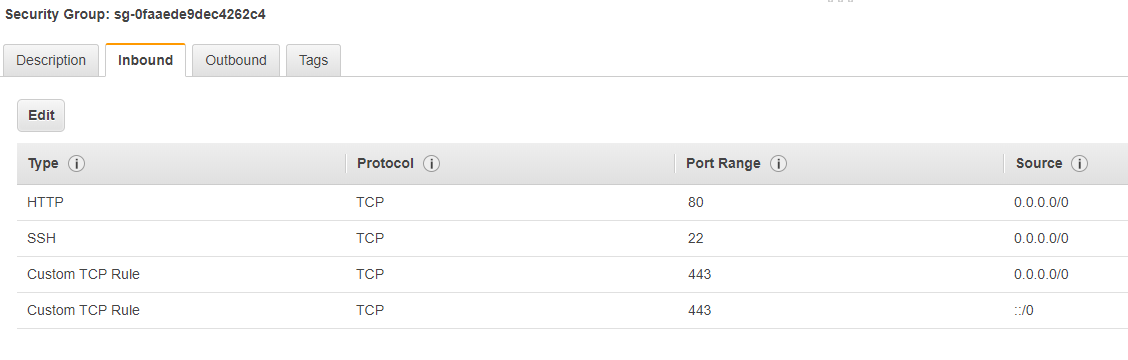
\includegraphics[width=\textwidth]{img/Security-Group}
	\caption{Firewall configuration for the instance}
	\label{fig:SecGroup}
\end{figure}

\subsubsection{MongoDB Setup}
At first we need to install MongoDB. Because the mongodb package provided by Ubuntu is not maintained by MongoDB\footnote{https://docs.mongodb.com/manual/tutorial/install-mongodb-on-ubuntu/}, we need to add the package-list and keyserver.
\begin{lstlisting}
sudo apt-key adv --keyserver hkp://keyserver.ubuntu.com:80 --recv 2930ADAE8CAF5059EE73BB4B58712A2291FA4AD5
echo "deb [ arch=amd64,arm64 ] https://repo.mongodb.org/apt/ubuntu xenial/mongodb-org/3.6 multiverse" | sudo tee /etc/apt/sources.list.d/mongodb-org-3.6.list
\end{lstlisting}

After that we can update the package-lists and install the official MongoDB package \textit{mongodb-org}.
\begin{lstlisting}
sudo apt-get update
sudo apt-get install -y mongodb-org
\end{lstlisting}

Now we can run the MongoDB daemon with
\begin{lstlisting}
sudo service mongod start
\end{lstlisting}

To automatically start the server while booting we can enable the service.
\begin{lstlisting}
sudo service mongod enable
\end{lstlisting}

\subsubsection{REST-Service Setup}
\label{sec:REST-Service}
The REST-Service is implemented in NodeJS\footnote{https://nodejs.org/en/}. Therefore we need to install NodeJS. This can be done using the following commands.
\begin{lstlisting}
curl -sL https://deb.nodesource.com/setup_8.x | sudo -E bash -
sudo apt-get install -y nodejs
\end{lstlisting}

As the REST-Service needs the following libaries:
\begin{enumerate}
	\item \textit{express} - a framework for routing
	\item \textit{body-parser} - to easily parse POST requests
	\item \textit{mongodb} - the connector to the DB
	\item \textit{geolib} - a framework for basic geometric computations.
\end{enumerate}
we need to install them with \textit{npm}.
\begin{lstlisting}
sudo npm install express --save
sudo npm install body-parser --save
sudo npm install mongodb --save
sudo npm install geolib --save
\end{lstlisting}

In order to provide the REST-Service as \textit{systemd} service we need to create the according file in the service directory (\textit{/etc/systemd/system/}). The contents of \textit{rest-client.service} are a brief description and the path to the location of the script.
\begin{lstlisting}
rest-client.service
[Unit]
Description=Rest Client

[Service]
ExecStart=/var/www/node/restaurant_client.js

[Install]
WantedBy=multi-user.target
\end{lstlisting}

The REST-Service should also be available upon boot, so we enable it as well.
\begin{lstlisting}
sudo systemctl enable rest-client
\end{lstlisting}

Because the script would need root privileges to run on any well-known port, but that is not favorable, we run the script on port 8000 and redirect all requests from port 80 to that port using \textit{iptables}.
\begin{lstlisting}
sudo iptables -t nat -D PREROUTING -p tcp --dport 80 -j REDIRECT --to-ports 8080
sudo iptables -t nat -D PREROUTING -p tcp --dport 443 -j REDIRECT --to-ports 8080
\end{lstlisting}
In order to persist the iptables rules we need to install the package \textit{iptables-persistent} and save the rules with the according command.
\begin{lstlisting}
sudo apt-get install iptables-persistent
service iptables save
\end{lstlisting}

\


\subsubsection{Android Setup}
\label{sec:Android-Setup}
This project is based on Android therefore the following software is necessary to build the project mobile client:

\begin{enumerate}
	\item \textit{Android Studio} - 3.1.2 - IDE for building Android projects
	\item \textit{Android SDK} - 27 for 8.1 Oreo - library for building apps
	\item \textit{Google Play  Services} - 49 - necessary for Google Places API
	\item \textit{Oracle JDK} - 8 - is necessary, because Android is based on Java/Kotlin
\end{enumerate}

All other necessary software for this project like a gradle wrapper or various third parties should be downloaded automatically, while the project is built by Android Studio.


\subsection{Datasets}

If you use any additional or different datasets than specified in the previous
section/checkpoint, name them and discuss their characteristics (as required in
the previous section/checkpoint) (min. 1 paragraph per dataset).

If you generated your own synthetic datasets and made changes to the generation
process described in the previous section/checkpoint, discuss and justify these
changes here (min. 1 paragraph per dataset).

\subsubsection{Generation}

If you generated your own synthetic datasets, explain in detail how your
datasets are generated (including code snippets). This includes (but is not
limited to) the programming language/tools and how you ensure that your datasets
satisfy the desired characteristics.

\subsubsection{Import}

Discuss the import process here (including code snippets). Did you apply any
transformations before the data is stored in the underlying database system?
Which information is (not) stored? How is the information represented in the
underlying data model of your system?

If your datasets are of static nature, how long did it take you to import the
datasets? Did you put some effort into optimizing the import process? If so,
reason about the necessity (for example, because of very long runtimes without
optimizations) and briefly describe why the optimizations did (not) improve your
import process (1 paragraph each).

\subsection{Implementation}

Describe the actual implementation of your application. This subsection is
supposed to summarize all important parts/modules of your implementation
(including code snippets). For example, if you use other frameworks/libraries,
describe how they interact with the remaining parts of your application.

This section (including its subsection) is supposed to constitue the majority
of the report which is also reflected in the gradine scheme. Hence, this part of
the report should at least be 2-3 pages in total (text \emph{and} figures).

\subsubsection{REST-Service}
The REST-Client is implemented in NodeJS as stated above. The libraries listed in section \ref{sec:REST-Service} help to get a small an well organized structure. The full code is available at Appendix section \ref{app:REST-Service}.

With \textit{express} you can create different routes for your server. Our application consists of three diferent routes. One is \textit{/getRestaurants}, where you get all restaurants which are in the database. This function was mainly used for debug purposes. The second and most important function is \textit{/getRestaurantsForLatLng}. This request is used by the Android-Client to get the current restaurants for its location. The thrid request is \textit{/createOrUpdateRestaurnt}. This is used by the crawler to update existing restaurants or create new ones. The different routes are generated by the following snippet.
\begin{lstlisting}
var app = express();
app.get('/getRestaurants', function (req, res) {
	...
});

app.post('/getRestaurantsForLatLngRad', function (req, res) {
	...
});

app.post('/createOrUpdateRestaurant', function (req, res) {
	...
});
\end{lstlisting}

A database connection can be established by using the MongoClient which is created the following way.
\begin{lstlisting}
var MongoClient = require('mongodb').MongoClient;
\end{lstlisting} 

The connection can then be created using the following snippet. After trying to connect you can check wheter that operation was successfull by checking the \textit{err} parameter.
\begin{lstlisting}
MongoClient.connect(url, function (err, client) {
	if (!err) {
		...
	}
});
\end{lstlisting}

The database and collection can be obtained in the following way.
\begin{lstlisting}
// Get DB
const db = client.db(dbName);

// Get the documents collection
const collection = db.collection(collectionName);
\end{lstlisting}

The collection can be queried using a JSON-Document as a filter. For example for checking if a restaurant is already in the database we use the following query.
\begin{lstlisting}
collection.find({ id: id }).toArray(function (err, docs) {
	if (!err) {
		if (docs.length == 0) { // new item
			...
		} 
	}
});
\end{lstlisting}

The location-aware request \textit{/getRestaurantForLatLngRad} makes it possible to provide the current location and a radius to look for restaurants in it. To check wheter a restaurant is in the given we range we use geolib's functionality \textit{geolib.isPointInCircle(...)}

The service to get the restaurants should be available to the public, but the create/update service should just be accesible from localhost. In order to achieve that, two servers are created, one for port 8080 (get) and and for port 8081 (create and update). As seen in section \ref{sec:setup}, HTTP(S) traffic is forwarded to port 8080, all other ports are blocked.
\begin{lstlisting}
http.createServer(app).listen(8080, function () {
	console.log('Server started on port 8080');
});

http.createServer(privateApp).listen(8081, function () {
	console.log('Private-Server started on port 8081');
});
\end{lstlisting}

\subsubsection{Android Application}

The application consists of three main visual interaction parts, a SQLite database and a http calling functionallity to communicate with the server. The following paragraphs will explain the most important parts.

\paragraph{UI - Restaurant Discovery}
The restaurant discovery is a visual snapshot of the devices SQLite database contents, therefore this means that all temporarely saved restaurants are visualised in a horizontal list. This list is swipeable and updates as the underlying database updates. This custom implementation is based on a horizontal Viewpager which is available from the Android-SDK.
\paragraph{UI - Place Selection}
The location selection lets the user select a location. This functionallity is based on the Google PlacePicker which returns pairs of latitude and longitude for each location. After the location has chosen, a fresh request is sent to the server and the restaurant list gets an update.
\paragraph{UI - Range Filters}
As range is important in terms of location, the user can select his desired search range in kilometers inside the 'Settings' tab. Based on the preferences the server query is altered and another dataset returned.
\paragraph{SQLite DB - Adapter Setup}
The SQLite database only consists of a single table for the restaurants. The most important fields like name, address, imageurl, etc.. are saved there. We have chosen an adapter setup where changes in the database lead to an immediate response in the UI components.
\paragraph{Network Calling}
Networking in Java is pretty simple, therefore we just open up a 'HttpURLConnection' to our server and make a post with the explained parameters. After that we parse the restaurant list which we get in response. With this list we fill the local Android database and notify all adapters about this update. 

\subsubsection{Key System Features}

Discuss at least two key features of your underlying (database) system that you
used to implement (or optimize) your application (min. 1 paragraph each). For
a bonus point, discuss two other features you found useful in your application
context.

This includes (but is not limited to) indexes, views, replication, sharding,
transactions, specialized algorithms or data structures, aggregations, \ldots

\subsection{Problems Encountered}

\emph{Optional}. If any, summarize problems your encountered while implementing
your application. Briefly describe how you resolved the respective problems.
Moreover, if you had to make design decisions, discuss and justify them here.

\subsection{Alternative Implementation}

\emph{Optional}. Describe an implementation of your application that is based on
a different (database/processing) system (1-2 paragraphs). Briefly specify the
key parts of this alternative implementation (1 paragraph each) and discuss the
main differences to your original implementation (for example, limitations,
advantages/disadvantages, any other interesting aspect with respect to
performance, scalability, flexbility, \ldots) (1 paragraph each).
